\documentclass[a4paper,12pt]{report}
\usepackage[utf8]{inputenc}
\usepackage[francais]{babel}
\usepackage{fancyhdr}
\usepackage{graphicx}
\usepackage{tikz}
\usetikzlibrary{calc}
\usepackage{listings}
\usepackage{xcolor}
\definecolor{grey}{rgb}{0.9,0.9,0.9}
\usepackage{titlesec}
\usepackage{verbatim}
\usepackage{listings}
\usepackage{textcomp}
\usepackage{hyperref}
\usepackage{longtable}
\usepackage{colortbl}
\usepackage{amssymb}


\frenchbsetup{StandardLists=true}
\newcommand{\marge}{18mm}
\usepackage[left=\marge,right=\marge,top=\marge,bottom=\marge]{geometry}
\pagestyle{fancy}
\setlength{\headheight}{14pt}
\chead{
  \textbf{Binôme :} Douaille Erwan 
    \hspace{2em}
  \textbf{Groupe :} M2 Info IVI}
\renewcommand{\headrulewidth}{1pt}
\linespread{1}
\setlength{\columnseprule}{0.2pt}
\definecolor{javakeyword}{rgb}{0,0,0.5}
\definecolor{javastring}{rgb}{0,0.5,0}
\definecolor{javacomment}{rgb}{0.5,0.5,0.5}
\lstdefinestyle{Scilab}{
   language=Scilab, basicstyle=\footnotesize,       % the size of the fonts that are used for the code
  numbers=left,                   % where to put the line-numbers
  numberstyle=\tiny\color{gray},  % the style that is used for the line-numbers
  stepnumber=1,                   % the step between two line-numbers. If it's 1, each line
                                  % will be numbered
  numbersep=5pt,                  % how far the line-numbers are from the code
  backgroundcolor=\color{white},  % choose the background color. You must add \usepackage{color}
  showspaces=false,               % show spaces adding particular underscores
  showstringspaces=false,         % underline spaces within strings
  showtabs=false,                 % show tabs within strings adding particular underscores
  frame=single,                   % adds a frame around the code
  rulecolor=\color{black},        % if not set, the frame-color may be changed on line-breaks within not-black text (e.g. commens (green here))
  tabsize=2,                      % sets default tabsize to 2 spaces
  captionpos=b,                   % sets the caption-position to bottom
  breaklines=true,                % sets automatic line breaking
  breakatwhitespace=false,        % sets if automatic breaks should only happen at whitespace
  title=\lstname,                 % show the filename of files included with \lstinputlisting;   stringstyle=\color{javastring},
   keywordstyle=\color{javakeyword}\ttfamily\textbf,
   commentstyle=\color{javacomment}\ttfamily\textit
 }
 

\begin{document}



\makeatletter
\begin{titlepage}
\centering
\vspace{-10em}
{\LARGE \textbf{\textsc{Rapport de Projet RVI}}}\\
\vspace{3em}

\includegraphics[scale=0.6]{image/thalassa.png}\\
\vspace{3em}
{\LARGE \textsc{Projet Thalassa: simulation de plongée sous-marine}}\\

\vspace{8em}
Par\\
\vspace{1em}
{\LARGE \@author}\\

\vspace{2em}



\begin{tikzpicture}[remember picture,overlay]

\node [below left,xshift=-1cm, yshift=4cm] at (current page.south east){
\includegraphics[scale=0.6]{image/ustl1.png}};

\end{tikzpicture}
\end{titlepage}
\makeatother

\sloppy

\setcounter{page}{1} 
\newpage

\section*{Introduction}

Dans ce tp nous allons découvrir la logique flou. La logique flou est une logique qui admet plusieurs degrés de réponse contrairement à la logique booléenne qui elle admet uniquement un vrai ou faux.


\subsection*{Fonctions d'appartenance}

Dans cette partie nous allons manipuler des ensembles flous. 

\begin{lstlisting}[style=Scilab,caption={Code question 1},label=lst:e1q1]
basse=zeros(1,40);
moyenne=zeros(1,40);
haute=zeros(1,40);
for i=1:10
    basse(i)=1;
end
for i=11:20
    basse(i)=1-(i-10)x0.1;
end
for i=11:20
    moyenne(i)=(i-10)x0.1;
end
for i=21:30
    moyenne(i)=1-(i-20)x0.1;
end    
for i=21:30
    haute(i)=(i-20)x0.1;
end
for i=31:40
    haute(i)=1;
end
\end{lstlisting}

Voici la création des ensembles. Pour les éléments compris entre 0 et 1 nous calculons la valeur. Le fait d'avoir des valeurs entre 0 et 1 est la différence que l'on peut trouver à la logique binaire. On admet qu'il y a des réponses possibles entre 0 et 1.
Ces ensembles sont ensuites affichés via ce programme:

\begin{lstlisting}[style=Scilab,caption={Code question 1},label=lst:e1q2]
function exercice1()
    clf();
    plot2d(basse, style=2);
    plot2d(moyenne, style=3);
    plot2d(haute, style=5);
endfunction
\end{lstlisting}

\newpage

Voici le graphique obtenue:

\begin{figure}[!ht]
	\center	
	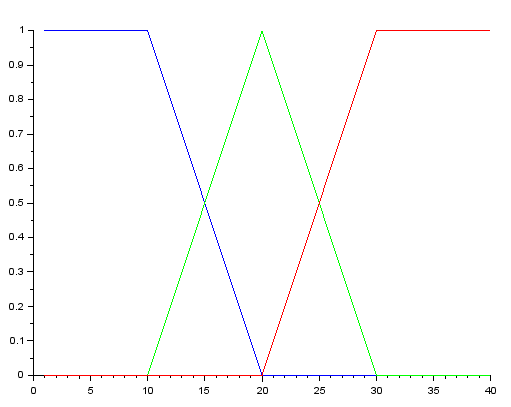
\includegraphics[scale=0.8]{image/e1-q1.PNG}
\end{figure} 

Pour une température mesurée de 16$^{\circ}$C les degrés d'appartenance sont


Le graphique pour l'ensemble flou "Température basse ou moyenne est le suivant":


\begin{figure}[!ht]
	\center	
	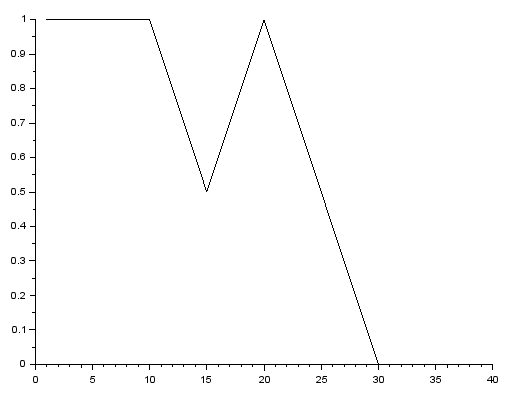
\includegraphics[scale=0.8]{image/e1-q2.PNG}
\end{figure} 

Pour obtenir ce graphique ils faut prendre le maximum des valeurs pour l'ensemble \textit{basse} et \textit{moyenne}.

\begin{lstlisting}[style=Scilab,caption={Code question 1.3},label=lst:e1q3]
    plot2d(1:40, max(basse,moyenne));
\end{lstlisting}

\newpage

\subsection*{Opérateurs de la logique flou}

Dans cette partie nous avons eu à réaliser 2 fonctions qui correspondent aux opérateurs \textit{min} et \textit{max}. Voici les fonctions Scilab nous permettant de réaliser ces opérateurs:

\begin{lstlisting}[style=Scilab,caption={Code question 2.1},label=lst:e2q1]    
function a=minFromE(e1, e2)
    len=length(e1);
    for i=1:len
        a(i)=min(e1(i),e2(i));
    end    
endfunction

function a=maxFromE(e1, e2)
    len=length(e1);
    for i=1:len
        a(i)=max(e1(i),e2(i));
    end
endfunction
\end{lstlisting}

Dans ces deux fonctions nous prenons deux ensembles et nous parcourons les valeurs pour obtenir le max ou le min de ces deux ensembles. Ces opérateurs sont semblables aux opérateurs logique \textit{ET} et \textit{OU}. Le min représentant le \textit{ET} (intersection) et le max représentant le \textit{OU} (union).

Voici un aperçu graphique de ces fonctions:

\begin{figure}[!ht]
	\center	
	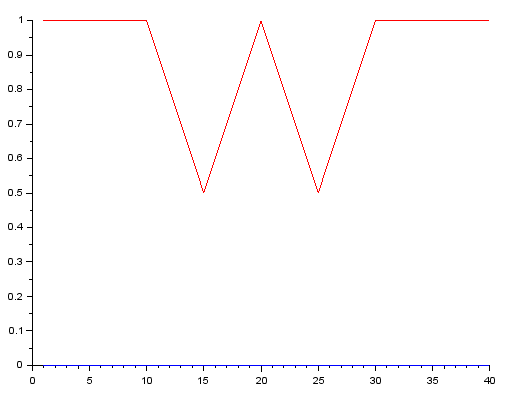
\includegraphics[scale=0.8]{image/e2-q1.PNG}
\end{figure} 

La courbe rouge représente le \textit{ET} des ensembles \textit{basse}, \textit{moyenne} et \textit{haute}, tandis que la bleu représente le \textit{OU} de ces mêmes sous-ensembles.

Et voici le code qui a permit de faire le rendu graphique:
\begin{lstlisting}[style=Scilab,caption={Code question 2.1},label=lst:e2q1]    
minimum=zeros(1,40);
maximum=zeros(1,40);    
minimum=minFromE(basse,moyenne);
minimum=minFromE(minimum,haute);
maximum=maxFromE(moyenne,haute);
maximum=maxFromE(maximum,basse);
plot2d(minimum, style=2);
plot2d(maximum, style=5);
\end{lstlisting}


\subsection*{Implication floue}

Dans cette dernière partie nous allons étudier la méthode d'implication floue de Mamdani. Cette méthode utilise le raisonnement par approximation, exemple en langage naturel, si la température est de 3$^{\circ}$C alors chauffer fort, si la température est de 8$^{\circ}$C alors chauffer un peu moins fort que pour 3$^{\circ}$C.

Le résultat de l'implication floue, dans notre exemple appliquée au chauffage en fonction de la température, est, comment je chauffe (fort ou non) en fonction de la température fournit en paramètre d'entrée.

Pour déterminer notre chauffe on a utilisé la méthode de Mamdani:
\begin{figure}[!ht]
	\center	
	\includegraphics[scale=0.5]{image/mamdani.png}
\end{figure} 

Dans notre cas le $\mu$\textit{prémisse(xO)} correspond à la pour 12$^{\circ}$C dans notre courbe basse, et le $\mu$\textit{conclusion(y)} correspond à la valeur en chauffer fort en fonction de la puissance de chauffe.

Voici le code ainsi que le graphique correspond à notre implémentation de la méthode de Mamdani:

\begin{lstlisting}[style=Scilab,caption={Code question 3},label=lst:e3]    
function exercice3(temp)
    clf();
    a=zeros(1,15);
    indice=basse(temp);
    for i=1:15
        a(i)=min(temperature(i), indice);
    end    
    
    plot2d(temperature, style=5);
    plot2d(a, style=2);
endfunction
\end{lstlisting}

\begin{figure}[!ht]
	\center	
	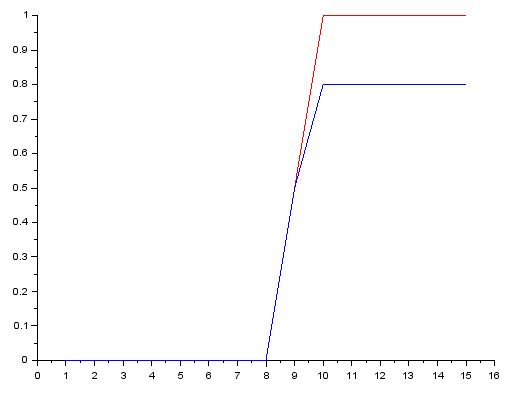
\includegraphics[scale=0.8]{image/e3-q1.PNG}
\end{figure} 

En rouge on à la courbe $\mu$\textit{conclusion(y)}. Ma courbe résultat en bleu n'est pas une droite entre 8 et 10. Cela est dûe au pas de mon tableau de température. Pour être plus précis j'aurais dû mettre un pas de 0.1 dans mon tableau pour obtenir des valeurs plus correctes et donc obtenir une droite.

En essayant avec d'autres valeurs comme 17$^{\circ}$C la courbe résultat est plus basse. C'est logique puisque à 17$^{\circ}$C il faut chauffer moins qu'a 12$^{\circ}$C en fonction de notre courbe de puissance de température.

\section*{Conclusion}

En conclusion nous avons eu une introduction à la logique floue. La logique floue permet d'exprimer avec plus de détails ce que la logique binaire aurait résolue en 2 résultats possibles. La logique floue est utilisée dans de nombreux domaines comme vue en cours avec les métros pour permettre une accélération/décélération plus douce pour les usagers.

\end{document}